\chapter{Tetis - Modelagem e Controle}


\section{Modelo}
O manipulador Tetis consiste basicamente de um braço planar de três elos com uma rotação adicional ao redor do eixo do plano. Também pode ser visto como um braço antropomórfico com uma junta de revolução adicional ao final da cadeia, com o eixo paralelo às duas anteriores. O projeto mecânico faz com que a extremidade do efetuador final não esteja exatamente alinhada com as juntas, o que é levado em conta no último elo. O esquema na figura \ref{fig:modelo_tetis} ilustra o modelo de elos e juntas. 
\begin{figure}[!ht]
\centering
  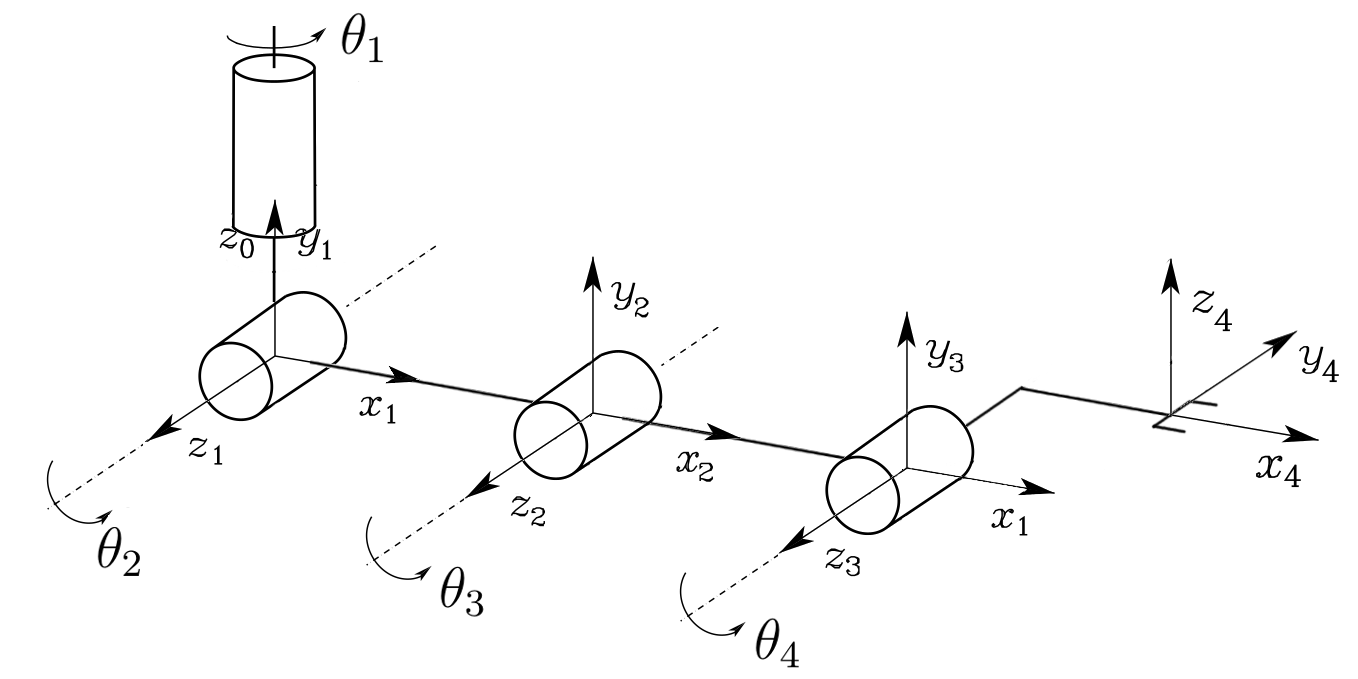
\includegraphics[width=0.9\linewidth]{./img/m2_meio_2.png}
  \caption{Modelagem do Manipulador Tetis e posicionamento dos sistemas de coordenadas}
  \label{fig:modelo_tetis}
\end{figure}%

\section{Cinemática Direta}
O primeiro passo ao modelar um manipulador robótico é encontrar a cinemática direta. Será utilizada a convenção de Denavit-Hartenberg para posicionar os sistemas de coordenadas e obter os parâmetros. Seguindo os passos descritos em \ref{sec:denavit} os sistemas de coordenadas foram posicionados da seguinte forma:

\begin{itemize}
\item Eixo $z_0$ escolhido ao longo da Junta 1. Origem $O_0$ escolhida arbitrariamente de modo a coincidir com $O_1$ por simplicidade.  
\item Eixo $z_1$ escolhido ao longo da Junta 2. Origem $O_1$ na intersecção entre $z_0$ e $z_1$. Eixo $x_1$ na direção normal ao plano definido por $z_0$ e $z_1$ pois se interceptam. O sentido foi arbitrariamente escolhido na direção de avanço da cadeia por simplicidade.
\item Eixo $z_2$ escolhido ao longo da Junta 3. Origem $O_2$ na junta 3 pois $z_2$ e $z_1$ são paralelas. Eixo $x_2$ escolhido arbitrariamente ao longo de  $x_1$ pois a normal comum entre $z_2$ e $z_1$ não é unicamente definida.
\item Eixo $z_3$ escolhido ao longo da Junta 4. Origem $O_3$ na junta 3 pois $z_3$ e $z_2$ são paralelas. Eixo $x_3$ escolhido arbitrariamente ao longo de  $x_2$ pois a normal comum entre $z_3$ e $z_2$ não é unicamente definida.
\item Como não existe junta 5, eixo $z_4$ definido arbitrariamente. Origem $O_4$ na extremidade do efetuador final. Eixo $x_4$ normal ao eixo $z_3$.
\end{itemize}

A partir dos eixos posicionados conforme a figura \ref{fig:modelo_tetis} é possível obter os parâmetros na tabela \ref{tab:dh_tetis}. 


\begin{table}[h!]
\centering
\caption{Parâmetros Denavit–Hartenberg para manipulatodor Tetis}
\label{tab:dh_tetis}
\begin{tabular}{rrrrr} \hline
Elo & $a_i$ & $\alpha_i$ & $d_i$  & $\theta_i$ \\ \hline
1   & 0     & $\pi/2$    & 0      & $\theta_1$ \\
2   & $E_3$ & 0          & 0      & $\theta_2$ \\
3   & $E_4$ & 0          & 0      & $\theta_3$ \\
4   & $E_5$ & $-\pi/2$   & $-M_5$ & $\theta_4$ \\ \hline
\end{tabular}
\end{table}


\begin{itemize}
\item $a_1 = 0$  e $d_1 = 0$ pois $O_0$ e $O_1$ coincidem. $\alpha_1 = \pi/2$ ângulo entre $z_0$ e $z_1$ ao redor de $x_i$.
\item $a_2 = E_3$ é a distância entre $z_1$ e $z_2$ ao longo de $x_2$ que corresponde ao comprimento do elo 2. $z_1$ e $z_2$ são sempre paralelos logo $\alpha_2 = 0$. A distância $d_2$ entre $x_1$ e $x_2$ ao longo de $z_1$ é zero. 

\item $a_3 = E_4$ é a distância entre $z_2$ e $z_3$ ao longo de $x_3$ que corresponde ao comprimento do elo 3. $z_2$ e $z_3$ são sempre paralelos logo $\alpha_3 = 0$. A distância $d_3$ entre $x_2$ e $x_3$ ao longo de $z_2$ é zero. 

\item $a_4 = E_5$ é a distância entre $z_3$ e $z_4$ ao longo de $x_4$. $\alpha_4 = -\pi/2$ é o ângulo entre $z_3$ e $z_4$ ao redor de $x_4$, sendo portanto negativo. $d_4 = -M_5$ é a distância entre $x_3$ e $x_4$ ao longo de $z_3$. 
\end{itemize}

Considerando a posição inicial da figura \ref{fig:modelo_tetis} todos os ângulos $\theta_i$ são dados diretamente pelas variáveis de junta, sem \textit{offsets}. 

A orientação de um sistema de coordenadas $i$ em relação ao anterior é dada por uma rotação de $\theta_i$ em torno de $z$ seguida de uma rotação em torno de $x$ de $\alpha_i$ considerando o sistema de coordenadas corrente.

\begin{equation}
\bm{R}_{i-1,i} = \bm{R}_z(\theta_i)\bm{R}_x(\alpha_i)
\end{equation}

A translação é obtida representando as distâncias no sistema de coordenadas $i-1$:
\begin{gather}
\bm{\vec{p}}_{i-1,i} = d_i \bm{\vec{z}}_{i-1} + a_i \bm{\vec{x}}_i \\
(\bm{\vec{p}}_{i-1,i})_{i-1} = d_i (\bm{\vec{z}}_{i-1})_{i-1} + a_i (\bm{\vec{x}}_i)_{i-1} \\
(\bm{\vec{p}}_{i-1,i})_{i-1} = d_i (\bm{\vec{z}}_{i-1})_{i-1} + a_i \bm{R}_{i-1,i}(\bm{\vec{x}}_i)_{i} 
\end{gather}

As duas informações podem ser representadas de uma forma mais compacta como transformação homogênea:
\begin{equation}
T_{i-1,i} = \m{
	R_{i-1,i} 		&  (\bm{\vec{p}}_{i-1,i})_{i-1} \\
	0_{1 \times 3}	&  							  1
}
\end{equation}
que em função dos parâmetros fica:
\begin{equation}
T_{i-1,i} = \m {
	c_{\theta_i}  & -s_{\theta_i}c_{\alpha_i}	&	s_{\theta_i}s_{\alpha_i}  &	a_i c_{\theta_i} \\ 
	s_{\theta_i}  &	c_{\theta_i}c_{\alpha_i}	&  -c_{\theta_i}s_{\alpha_i}  & a_i s_{\theta_i} \\
	0			  & s_{\alpha_i}				&   c_{\alpha_i}			  &	d_i				 \\
	0			  & 0							&   0						  & 1
}
\end{equation}

Obtemos então:
%\begin{align*}
%\bm{R}_{01} =
%\m{c_1 & 0 & s_1   \\
%   s_1 & 0 & -c_1  \\
%   0   & 1 &    0  \\} 
%& & \vec{\bm{p}}_{01} = 0
%\end{align*}
%\begin{align*}
%R_{12} = 
%\m{c_2 & -s_2 &  0  \\
%   s_2 &  c_2 &  0  \\
%   0   &    0 &  1  \\} 
%\end{align*}
%\begin{align*}
%R_{23} = 
%\m{c_3 & -s_3 &  0  \\
%   s_3 &  c_3 &  0  \\
%   0   &    0 &  1  \\} 
%\end{align*}
%\begin{align*}
%R_{34} = 
%\m{c_4 &  0 & -s_4  \\
%   s_4 &  0 &  c_4  \\
%   0   & -1 &    0  \\} 
%\end{align*}


%\begin{equation}
%\bm{R}_{04} = 
%\m{
%	c_1 c_{234} & -s_1 & -c_1 s_{234} \\
%	s_1 c_{234} & -c_1 & -s_1 s_{234} \\
%		s_{234} &    0 & 	  c_{234}
%}
%\end{equation}

\begin{align*}
\bm{T}_{01} = 
\m{c_1 & 0 & s_1 &  0 \\
   s_1 & 0 & -c_1 & 0 \\
   0   & 1 &    0 & 0 \\
   0   & 0 &    0 & 1}
& &
\bm{T}_{12} =  \m{c_2 & -s_2 &  0 & E_3 c_2 \\
   s_2 &  c_2 &  0 & E_3 s_2  \\
   0   &    0 &  1 & 	   0  \\
   0   &    0 &  0 &       1} 
\end{align*}

\begin{align*}
\bm{T}_{23} = 
\m{c_3 & -s_3 &  0 & E_4 c_3 \\
   s_3 &  c_3 &  0 & E_4 s_3  \\
   0   &    0 &  1 & 	   0  \\
   0   &    0 &  0 &       1}
& &
\bm{T}_{34} = 
\m{c_4 &    0 &  -s_4 & E_5 c_4 \\
   s_4 &    0 &   c_4 & E_5 s_4 \\
   0   &   -1 &     0 & 	-M_5 \\
   0   &    0 &     0 &       1}
\end{align*}


\begin{equation} \label{eq:cine_direta}
 \bm{T}_{04} = \bm{T}_{01} \bm{T}_{12}  \bm{T}_{23} \bm{T}_{34} = 
\m{
   c_1 c_{234} & -s_1 & -c_1 s_{234} & -M_5 s_1 + E_4 c_{23}c_1 + E_3 c_1 c_2 + E_5 c_{234} c_1 \\
   s_1 c_{234} & -c_1 & -s_1 s_{234} &   M_5 c_1+E_4 c_{23} s_1 + E_3 c_2 s_1 + E_5 c_{234} s_1 \\
   s_{234}     &    0 &      c_{234} &					     E_4 s_{23} + E_3 s_2 + E_5 s_{234} \\
   0   &    0 &     0 &      												   1
} 
\end{equation}

\section{Espaço das Juntas e Operacional}
Antes de tratar de estratégias de controle é necessário definir o espaço operacional e o espaço das juntas,  sob os quais serão aplicadas as leis de controle. 
Como trata-se de um manipulador 4-DOF de temos que o vetor do espaço operacional tem dimensão $(4 \times 1)$ dado por 
\begin{equation}
\bm{x_e} = \m{\bm{p}_e \\ \phi_e}
\end{equation}
onde o vetor $\bm{p}_e$ descreve a posição cartesiana representada no referencial da base:
\begin{equation}
\bm{p}_e = \m{x \\ y \\ z}
\end{equation}
e $\phi_e$ é o grau de liberdade de orientação \textit{pitch} no referencial do efetuador (??), dado por
\begin{equation} \label{eq:orientacao}
\phi_e = -(\theta_2 + \theta_3 + \theta_4)
\end{equation}

O espaço das juntas é definido por 
\begin{equation} \label{joint_space}
\bm{q} = \m{q_1 \\ q_2 \\ q_3 \\ q_4} = \m{\theta_1 \\ \theta_2 \\ \theta_3 \\ \theta_4  }
\end{equation} 
pois todas as juntas são de revolução.

\section{Cinemática Diferencial}

\subsection{Jacobiano Analítico}
A partir da cinemática direta em \eqref{eq:cine_direta} e da equação \ref{eq:jacob_pos} podemos obter o Jacobiano de Posição para o manipulador diferenciando a equação em relação as variáveis de junta. \cite{book-example}

\begin{equation}
\bm{p}_e = \m{x \\ y \\ z} =
\m{
   -M_5 s_1 + E_4 c_{23}c_1 + E_3 c_1 c_2 + E_5 c_{234} c_1 \\
     M_5 c_1+E_4 c_{23} s_1 + E_3 c_2 s_1 + E_5 c_{234} s_1 \\
   						 E_4 s_{23} + E_3 s_2 + E_5 s_{234} \\
}
\end{equation}

\begin{equation}
(\bm{J}_P)_0 = 
\m{
	\ddfrac{\partial x}{\partial q_1} & \ddfrac{\partial x}{\partial q_2} & \ddfrac{\partial x}{\partial q_3} & \ddfrac{\partial x}{\partial q_4}  \\
	\ddfrac{\partial y}{\partial q_1} & \ddfrac{\partial y}{\partial q_2} & \ddfrac{\partial y}{\partial q_3} & \ddfrac{\partial x}{\partial q_4}  \\
	\ddfrac{\partial z}{\partial q_1} & \ddfrac{\partial z}{\partial q_2} & \ddfrac{\partial z}{\partial q_3} & \ddfrac{\partial z}{\partial q_4}  \\
}
\end{equation}
onde
\begin{align*}
&\frac{\partial x}{\partial q_1} =& - M_5c_1 - E_4c_{23}s_1 - E_3c_2s_1 - E_5c_{234}s_1  \\
&\frac{\partial x}{\partial q_2} =& -c_1(E_4s_{23}+E_3s_2+E_5s_{234}) \\
&\frac{\partial x}{\partial q_3} =& -c_1(E_4s_{23}+E_5s_{234}) \\
&\frac{\partial x}{\partial q_4} =& -E_5s_{234}c_1 \\
&\frac{\partial y}{\partial q_1} =& -M_5s_1+E_4c_{23}c_1+E_3c_1c_2+E_5c_{234}c_1 \\
&\frac{\partial y}{\partial q_2} =& -s_1(E_4s_{23}+E_3s_2+E_5s_{234}) \\
&\frac{\partial y}{\partial q_3} =& -s_1(E_4s_{23}+E_5s_{234}) \\
&\frac{\partial y}{\partial q_4} =& -E_5s_{234}s_1 \\ 
&\frac{\partial z}{\partial q_1} =& 0 \\ 
&\frac{\partial z}{\partial q_2} =& E_4c_{23}+E_3c_2+E_5c_{234} \\
&\frac{\partial z}{\partial q_3} =& E_4c_{23}+E_5c_{234}\\
&\frac{\partial z}{\partial q_4} =& E_{5}c_{234} 
\end{align*}

A partir de \ref{eq:jacob_or} e de \ref{eq:orientacao} podemos calular o Jacobiano de Orientação
\begin{equation}
\bm{J}_{\phi}(\bm{q}) = \frac{\partial \phi_e}{\partial \bm{q}} = \m{0 & -1 & -1 & -1}
\end{equation}
 
Em alguns modos como controle por servo visão e no controle manual com joystick é interessante fazer o controle no referencial do efetuador, portanto precisamos representar o Jacobiano de posição no referencial do efetuador como $(\bm{J}_P)_N = \bm{R}_{04}^T (\bm{J}_P)_0$.  

\begin{equation}
(\bm{J}_P)_N =  
\m{
    -M_5c_{234} & E_3s_{34}+E_4s_4 & E_4s_4 & 0 \\
    E_4c_{23}+E_3c_2+E_5c_{234} & 0 & 0 & 0 \\
    M_5s_{23} &  E_5+E_3c_{34}+E_4c_4 & E_5+E_4c_4 & E_5 
}
\end{equation}

A partir daqui, para simplificar a notação, sempre será referenciado o Jacobiano Analitico no referencial da base $(\bm{J}_A)_0$  como  $\bm{J}_0$ e o Jacobiano Analítico no referencial do efetuador $(\bm{J}_A)_N$ como $\bm{J}_N$.

%\section{Singularidades}

\section{Modos de Controle}
\subsection{Velocidade no Espaço Operacional}
Este é um modo em malha aberta, onde o sinal de entrada no controlador é de velocidade no referencial da base ou do efetuador, ou seja a velocidade linear $\bm{\dot{p}}_d$. Utiliza-se a equação \eqref{eq:jacob_pos} para calcular a velocidade de cada junta. 

\begin{figure}[h!]
\centering
\begin{tikzpicture}[auto, node distance=2cm,>=latex']
    % We start by placing the blocks
    \node [input, name=input] {};
    \node [block, right of=input] (J) {$J^{-1}$};
    \node [block, right of=J] (Integral) {$\int$};
    \node [output, right of=Integral] (output) {};

    \draw [draw,->] (input) -- node {$\dot{\bm{x}}_e$} (J);
    \draw [->] (J) -- node {$\bm{\dot{q}}$} (Integral);
    \draw [->] (Integral) -- node [name=x] {$\bm{q}$}(output);
\end{tikzpicture}
\caption{Diagrama de Blocos: Modo de velocidade do Espaço Operacional}
\label{fig:vel_op}
\end{figure}


\subsubsection{Base}
Quando escolhe-se o referencial da base $\bm{\dot{x}}_d$ é velocidade desejada expressa no referencial da base e utiliza-se $J_0$.
\begin{equation}
\bm{u} = \bm{\dot{q}}_d = \bm{J}_0^{-1} (\bm{\dot{x}}_d)_0
\end{equation}
\subsubsection{Efetuador}
Quando escolhe-se o referencial da efetuador $\bm{\dot{x}}_d$ é velocidade desejada expressa no referencial do efetuador e utiliza-se $J_N$.
\begin{equation}
\bm{u} = \bm{\dot{q}}_d = \bm{J}_N^{-1} (\bm{\dot{x}}_d)_N
\end{equation}
onde 
\begin{equation}
\bm{\dot{x}}_d = \m{\bm{\dot{p}}_d \\ 0}
\end{equation}

\subsection{Posição no Espaço das Juntas}
O controle de posição no espaço das juntas consiste em uma realimentação com controle proporcional individual para cada junta. Considerando que as juntas sejam modeladas como integradores, o diagrama \ref{fig:pos_juntas} mostra a malha de controle.

\begin{figure}[h!]
\centering
\begin{tikzpicture}[auto, node distance=2cm,>=latex']
    % We start by placing the blocks
    \node [input, name=input] {};
    \node [sum, right of=input] (sum) {};
    \node [block, right of=sum] (controller) {$K_j$};
    \node [block, right of=controller] (system) {$\ddfrac{1}{s}$};
    % We draw an edge between the controller and system block to 
    % calculate the coordinate u. We need it to place the measurement block. 
    \draw [->] (controller) -- node[name=u] {$\bm{u}$} (system);
    \node [output, right of=system] (output) {};
    \node [tmp, below of=u] (tmp1) {};

    % Once the nodes are placed, connecting them is easy. 
    \draw [->] (system) -- node [name=s] {$\bm{q}$}(output);
    \draw [draw,->] (input) -- node {$\bm{q_d}$} (sum);
    \draw [->] (sum) -- node {$\bm{e}$} (controller);
    \draw [->] (s) |- (tmp1)-| node[pos=0.99] {$-$} node [near end] {$\bm{q}$} (sum);
       %\draw [->] (measurements) -| node[pos=0.99] {$-$} 
       % node [near end] {$\bm{q}_m$} (sum);
\end{tikzpicture}
\caption{Diagrama de Blocos: Modo de Posição no Espaço das Juntas}
\label{fig:pos_juntas}
\end{figure}

A lei de controle é dada por 
\begin{equation}
\bm{u} = \bm{K}_j (\bm{q}_d - \bm{q})
\end{equation}
onde 
\[ K_j = \m {
	k_j & 0 & 0 \\ 
	0 & k_j & 0 \\ 
	0 &  0  & k_j
}
\]

\subsection{Posição no Espaço Operacional}
Para este modo considera-se o problema de controle de posição no espaço operacional conforme definido em \ref{eq:op_space}. 

\subsection{Rastreamento de Trajetória}
Para o rastreamento de trajetória considera-se o problema de seguir um referência no referencial da base $\bm{x}_d(t)$ que é função do tempo, conhecidos $\bm{x}_d(t)$ e $\bm{\dot{x}}_d(t)$. Conforme mostrado em \ref{controle_cinematico}, a lei de controle dada por 
\begin{equation}
\bm{u} = \bm{J}_0^{-1}(\bm{q}) (\dot{\bm{x}}_d + \bm{K}_t (\bm{x_d} - \bm{x}))
\end{equation} 
é capaz de levar o erro assintoticamente a zero pois a dinâmica fica 
\begin{equation}
\dot{\bm{e}} + \bm{K} \bm{e} = 0
\end{equation}


\subsection{Servo Visão}


\subsection{Força}
\subsubsection{Float}

\subsubsection{Approach}
Considera-se o problema de controle de força na direção de \textit{approach} para o manipulador robótico 4-DOF em questão. A realimentação de força é feita com o uso do sensor descrito em \ref{sec:sensor_forca}. O objetivo de controle é rastrear uma entrada na forma de um degrau de força, a ser aplicada em uma placa de poliestireno montada em um suporte fixado na vertical como mostra a figura \ref{fig:suporte_forca}.  

É possível modelar o ambiente (força de contato), ou seja, a placa de poliestireno, como uma mola linear, através da \textit{Lei de Hooke}: \cite{bib:toni}
\begin{equation}
f = -k_s (x - x_s)
\end{equation}
onde $x$ é a posição do ponto de contato com a superfície e $x_s$ um ponto na superfície.

Foi feito um ensaio para encontrar a constante $k_s$ variando a distância $x_s$ e medindo a força resultante. Os dados experimentais e a regressão linear pode ser vista na figura \ref{fig:ks_linreg}. A constante encontrada foi $k_s = 379.7642 N/m$.

\begin{figure}[!ht]
\centering
  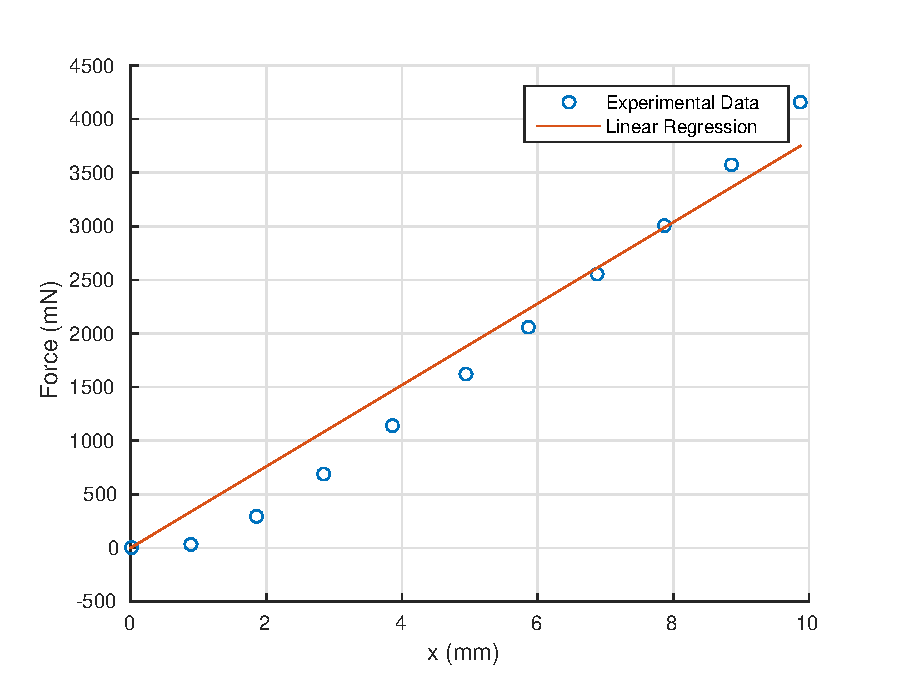
\includegraphics[width=0.5\linewidth]{./img/ks_estimation.eps}
  \caption{Trajetória}
  \label{fig:ks_linreg}
\end{figure}%


Considerando que o controle de força seja ativado somente após a etapa de contato com o ambiente onde será aplicada a força e que o controle de força é feito apenas na direção de approach (segundo o referencial do manipulador, na direção $x$), pode-se utilizar a malha de controle mostrada na figura \ref{fig:controle_forca}.

É utilizada uma lei de controle com ação proporcional e integral:
\begin{equation}
u = -K_s^{-1} (K_fe_f + K_i \int_0^t e_f(\tau)d\tau)
\end{equation}


\begin{figure}[h!]
\centering
\begin{tikzpicture}[auto, node distance=2cm,>=latex']
    % We start by placing the blocks
    \node [input, name=input] {};
    \node [sum, right of=input] (sum) {};
    \node [block, right of=sum] (Ks1) {$k_s^{-1}$};
    \node [block, right of=Ks1] (C) {$C(s)$};
    \node [blockbig=right:C] (J) [right=1cm of C] {$J_N^{-1}$};
    \node [block=right:J] (Integral) [right=1cm of J] {$\int$};
    \node [blockbig, right of=Integral] (DirKine) {$\bm{k}(\cdot)$};

	\node [tmp=below:J] (tmp0) [below left=-1.25cm and .7cm of J] {};
	\node [tmp=below:J] (tmp00) [below left=-2cm and 0.7cm of J] {};
	\node [tmp=below:J] (tmp000) [below left=-2cm and 0cm of J] {};

    \node [tmp=below:J] (tmp1) [below left=-1.5cm and 0.5cm of J] {};
    \node [tmp=below:J] (tmp2) [below left=-1.5cm and 0cm of J] {};

    \node [tmp=below:J] (tmp3) [below left=-1cm and 0.5cm of J] {};
    \node [tmp=below:J] (tmp4) [below left=-1cm and 0cm of J] {};

    \node [tmp=below:J] (tmp5) [below left=-0.5cm and 0.5cm of J] {};
    \node [tmp=below:J] (tmp6) [below left=-0.5cm and 0cm of J] {};

    \node [tmp=below:J] (tmpk0) [below right=-2cm and 0cm of DirKine] {};
	\node [tmp=below:J] (tmpk00) [below right=-2cm and 0.7cm of DirKine] {};
	\node [tmp=below:J] (tmpk000) [below right=-1.25cm and 0.7cm of DirKine] {};

    \node [tmp=below:J] (tmpk1) [below right=-1.5cm and 0.5cm of DirKine] {};
    \node [tmp=below:J] (tmpk2) [below right=-1.5cm and 0cm of DirKine] {};

    \node [tmp=below:J] (tmpk3) [below right=-1cm and 0.5cm of DirKine] {};
    \node [tmp=below:J] (tmpk4) [below right=-1cm and 0cm of DirKine] {};

    \node [tmp=below:J] (tmpk5) [below right=-0.5cm and 0.5cm of DirKine] {};
    \node [tmp=below:J] (tmpk6) [below right=-0.5cm and 0cm of DirKine] {};


    \node [block=right:DirKine] (ks) [right=1cm of DirKine] {$k_s$};
    \node [output, right of=ks] (output) {};

    % Once the nodes are placed, connecting them is easy. 
    \draw [draw,->] (input) -- node {$f_d$} (sum);
    \draw [->] (sum) -- node {$e_f$} (Ks1);
    \draw [->] (Ks1) -- node {} (C);
    %\draw [->] (C) -- node[name=u] {$u$} (tmp0);
    \draw [->] (J) -- node {$\bm{\dot{q}}$} (Integral);
    \draw [->] (Integral) -- node {$\bm{q}$} (DirKine);
    \node [block, below of=J] (measurements) {$H(s)$};
    %draw [->] (DirKine) -- node {} (ks);
    \draw [->] (ks) -- node [name=x] {$f$}(output);
    \draw [->] (x) |- (measurements);
    \draw [->] (measurements) -| node[pos=0.99] {$-$} 
        node[near end] {$f_m$} (sum);

    \draw [->] (C) -- (tmp0) -|  (tmp00) |- node[pos=0.65] {$x$} (tmp000);

    \draw [->] (tmpk0) -- node[pos=0.2] {$x$} (tmpk00) -|  (tmpk000) |-  (ks);
    \draw [->] (tmp1) -- node[pos=0] {$y$} (tmp2);
    \draw [->] (tmp3) -- node[pos=0] {$z$} (tmp4);
    \draw [->] (tmp5) -- node[pos=0] {$\phi$} (tmp6);

    \draw [->] (tmpk2) -- node[pos=0.3] {$y$} (tmpk1);
    \draw [->] (tmpk4) -- node[pos=0.3] {$z$} (tmpk3);
    \draw [->] (tmpk6) -- node[pos=0.3] {$\phi$} (tmpk5);
    %\draw [->] (x) |- (tmp1) -| node[pos=0.9] {$-$} (sum);
\end{tikzpicture}
\caption{Diagrama de Blocos: Malha de Controle de Força.}
\label{fig:controle_forca}
\end{figure}

O diagrama \ref{fig:controle_forca} pode ser simplificado se abstrairmos as outras dimensões que não a de approach, resultando em \ref{fig:controle_forca_simples}.

\begin{figure}[h!]
\centering
\begin{tikzpicture}[auto, node distance=2cm,>=latex']
    % We start by placing the blocks
    \node [input, name=input] {};
    \node [sum, right of=input] (sum) {};
    \node [block, right of=sum] (Ks1) {$k_s^{-1}$};
    \node [block, right of=Ks1] (C) {$C(s)$};
    \node [block, right of=C] (PWM) {$k_s$};
    \node [block, right of=PWM] (Robo) {$\ddfrac{1}{s}$};
    \node [tmp, below of=K] (tmp1){};
    \node [output, right of=Robo] (output) {};

    % Once the nodes are placed, connecting them is easy. 
    \draw [draw,->] (input) -- node {$f_d$} (sum);
    \draw [->] (sum) -- node {$e_f$} (Ks1);
    \draw [->] (Ks1) -- node {} (C);
    \draw [->] (C) -- node[name=u] {$u$} (PWM);
    \node [block, below of=u] (measurements) {$H(s)$};
    \draw [->] (PWM) -- node [name=tau] {} (Robo);
    \draw [->] (Robo) -- node [name=x] {$f$}(output);
    \draw [->] (x) |- (measurements);
    \draw [->] (measurements) -| node[pos=0.99] {$-$} 
        node[near end] {$f_m$} (sum);
    %\draw [->] (x) |- (tmp1) -| node[pos=0.9] {$-$} (sum);
\end{tikzpicture}
\caption{Diagrama de Blocos: Malha de Controle de Força Simplificada.}
\label{fig:controle_forca_simples}
\end{figure}

Considerando $H(s) = 1$
\begin{equation}
G(s) = \frac{k_p s + k_i}{s^2 + k_p s + k_i}
\end{equation}

Como o sinal vindo do sensor é bastante ruidoso, utiliza-se um filtro de primeira ordem com $f_c = 1$.
\begin{equation}
H(s) = \frac{1}{\tau s + 1}
\end{equation}
onde $\tau = 1/(2 \pi f_c) = 0.159154943$.

\begin{equation}
G(s) = \frac{k_p \tau s^2 + (k_p + \tau k_i)s + k_i}{\tau s^3 + s^2 + k_p s + k_i}
\end{equation}

%Especificações:


\subsubsection{Híbrido}
Considerando o diagrama \ref{fig:controle_forca}, é possível suprir os graus de liberdade não controlados $y$, $z$ e $\phi$ com outra lei de controle, como por exemplo o um Proporcional com Feedforward de modo a aplicar uma força na direção de approach e traçar uma trajetória de na superfície em que a força está sendo aplicada. 


\subsection{Master-Slave (Omni)}
TODO

% TODO: TABELA COM LEIS DE CONTROLE E FONTE DOS DADOS 